% LaTeX template for "A Comparative Study of Game-Theoretic and Reinforcement Learning Approaches for Jam-Resilient Wireless Networks in IoT"
\documentclass[conference]{IEEEtran}
%======================== Packages ========================
\usepackage{amsmath,amssymb}
\usepackage{graphicx}
\usepackage{algorithm,algpseudocode}
\usepackage{cite}
\usepackage{url}
\usepackage{booktabs} 
\usepackage[utf8]{inputenc} 
\usepackage[T1]{fontenc}  
\usepackage{microtype}
\usepackage[hidelinks]{hyperref}

\graphicspath{{figures/}} 

\begin{document}

%======================== Title and Authors ========================
\title{A Comparative Study of Game-Theoretic and Reinforcement Learning Approaches for Jam-Resilient Wireless Networks in IoT}

\author{
  \IEEEauthorblockN{Muhammad Umar Yaksambi}
  \IEEEauthorblockA{
    Dept. of CSE (Data Sciences)\\
    RV College Of Engineering\textregistered\\
    Bengaluru, India\\
    Email: mumaryaksambi.cd23@rvce.edu.in
  }
  \and
  \IEEEauthorblockN{Anuj Devpura}
  \IEEEauthorblockA{
    Dept. of CSE (Data Sciences)\\
    RV College Of Engineering\textregistered\\
    Bengaluru, India\\
    Email: anujdevpura.cd23@rvce.edu.in
  }
  \and
  \IEEEauthorblockN{Sadashiv Todakar}
  \IEEEauthorblockA{
    Dept. of CSE (Data Sciences)\\
    RV College Of Engineering\textregistered\\
    Bengaluru, India\\
    Email: sadashivtodakar.cd23@rvce.edu.in
  }
  \and
  \IEEEauthorblockN{Dr. Chethana R Murthy}
  \IEEEauthorblockA{
    Dept. of CSE \\
    RV College Of Engineering\textregistered\\
    Bengaluru, India\\
    Email: chethanamurthy@rvce.edu.in
  }
  \and
  \IEEEauthorblockN{Dr. Nagaraja G.S}
  \IEEEauthorblockA{
    Dept. of CSE \\
    RV College Of Engineering\textregistered\\
    Bengaluru, India\\
    Email: nagarajags@rvce.edu.in
  }
}

\maketitle

%======================== Abstract ========================
\begin{abstract}
This paper presents a comparative analysis of two adaptive defense strategies against jamming in wireless Internet-of-Things (IoT) networks: a Bayesian game-theoretic framework and a Q-Learning–based reinforcement learning (RL) approach. Designed for resource-constrained IoT environments, both strategies are evaluated for their effectiveness in mitigating jamming attacks.

Simulations are conducted on Erd\H{o}s–R\'enyi network topologies ($n = 10$, $p = 0.4$) over 500 time steps and five independent trials. Key performance metrics include attacker and defender payoffs, detection rate, and overall network health. Matchup matrices, convergence curves, and statistical validation via ANOVA ($p < 0.001$) are used to assess performance across strategy combinations.

Results show that Bayesian defenders outperform Q-Learning counterparts with a 7.3\% higher detection rate, a 10.2\% lower attacker payoff, and a 5.9\% improvement in network health on average. While Q-Learning enables faster early adaptation, it exhibits greater variability and a tendency to converge to suboptimal policies.

The findings reveal a clear trade-off between learning adaptability and performance stability. Bayesian strategies offer robust, consistent outcomes, making them suitable for predictable defense, while Q-Learning provides reactive flexibility. These insights inform the design of hybrid defenses for future IoT applications. The complete simulation framework is publicly available.
\end{abstract}

%======================== Keywords ========================
\begin{IEEEkeywords}
IoT security, jamming defense, game theory, reinforcement learning, Q-Learning, Bayesian games, network resilience
\end{IEEEkeywords}

%======================== 1. Introduction ========================
\section{Introduction}

As wireless Internet-of-Things (IoT) networks proliferate across smart infrastructure, healthcare, and consumer environments, they face growing exposure to jamming attacks that exploit the broadcast nature of shared frequency channels \cite{survey2022jamming}. By injecting interference signals, adversaries can disrupt communication, degrade throughput, and cause mission-critical failures. These threats are particularly concerning in IoT systems, which often operate under tight constraints on energy, memory, and computational capacity \cite{singh2023bayesian}.

Recent studies have emphasized the rising complexity of jamming techniques in evolving communication ecosystems like 5G/6G and industrial IoT, necessitating more intelligent countermeasures \cite{lohan2024ai, bensaad2023jamming}. While simple techniques like channel hopping offer limited protection against static jammers, they fall short against adaptive adversaries. To address this, game-theoretic models have been proposed to anticipate attacker behavior through strategic reasoning \cite{jia2022game}. However, such models rely on predefined payoff structures and may underperform when network dynamics evolve unpredictably. On the other hand, reinforcement learning (RL) offers adaptive defense via trial-and-error policy optimization \cite{tang2024adaptive}, but it can require substantial exploration and may converge to suboptimal strategies—especially in noisy or sparse-reward environments.

In this paper, we present a head-to-head evaluation of a Bayesian game-theoretic defense and a Q-Learning–based RL defense, both implemented within a common simulation framework. We address the following research questions:
\begin{enumerate}
  \item How do average attacker and defender payoffs, detection rates, and network health compare across strategies?  
  \item What are the convergence behaviors and stability characteristics of the learned policies?  
  \item Are the observed differences in performance statistically significant?  
\end{enumerate}

Our contributions are as follows:
\begin{itemize}
  \item We design and implement a modular simulation framework supporting interchangeable attacker and defender strategies.  
  \item We visualize strategy matchups using heatmaps for key performance metrics including payoff, detection rate, and network health.  
  \item We conduct rigorous statistical evaluation using one-way ANOVA to confirm performance differences across strategies.  
  \item We analyze the trade-offs between stability and adaptability, and propose future hybrid defense mechanisms that combine Bayesian and RL strengths.  
\end{itemize}

%======================== 2. Related Work ========================
\section{Related Work}

\subsection{Game-Theoretic Jamming Defense}
Game theory has been extensively applied to anti-jamming, modeling frequency selection as a two-player zero-sum or non-zero-sum game. Early work by Axell et al. \cite{axell2012detection} proposes Nash equilibrium strategies for frequency hopping, while Chen and Tong \cite{chen2019anti} incorporate energy constraints. Bayesian games extend this framework to handle incomplete information about attacker capabilities, improving robustness \cite{alpcan2007game,khouzani2012evolving}. Recent developments include Stackelberg models and healthcare-oriented applications, such as Gouissem et al.'s Nash game-based power allocation strategy for jam-resilient healthcare IoT \cite{gouissem2022nash} and Imran et al.'s Stackelberg game leveraging DSSS for anti-jamming in cognitive radio networks \cite{imran2024stackelberg}. Barkatsa et al. \cite{barkatsa2024bayesian} propose a Bayesian game-theoretic uplink allocation method tailored for federated IoT under jamming scenarios. Jia et al. \cite{jia2022game} further demonstrate game-theoretic learning approaches for anti-jamming in wireless networks, while Singh and Gupta \cite{resource2023slicing} explore game theory applications in B5G resource allocation. However, the computational complexity grows rapidly with network size and action space.

\subsection{Reinforcement Learning for Security}
Reinforcement learning offers a dynamic alternative, enabling agents to learn channel-selection policies without explicit attacker modeling. Peng et al. \cite{peng2017anti} apply Q-Learning to anti-jamming, achieving significant throughput improvements, while Luo et al. \cite{luo2018anti} leverage deep RL for spectrum sharing. Rahman et al. \cite{rahman2023rlbased} propose a multi-agent game-theoretic framework for RL-based attack detection in IoT networks, demonstrating the potential of hybrid approaches. Tang et al. \cite{tang2024adaptive} show adaptive anti-jamming strategies for UAV-aided IoT communications using reinforcement learning. Li et al. \cite{li2022drl} propose a DRL-based scheme for joint frequency and power control in dynamic wireless links, showing promising anti-jamming performance under fluctuating network conditions. Hybrid approaches combining game theory and RL have emerged, demonstrating enhanced performance \cite{zhao2020hybrid,li2021game}.

\subsection{Comparative Analyses}
Comparisons between game-theoretic and RL-based defenses are scarce. Zhao et al. \cite{zhao2020hybrid} evaluate hybrid schemes but focus on throughput only. Comprehensive surveys \cite{survey2022jamming} highlight the need for systematic comparisons across multiple performance dimensions. Our study distinguishes itself by evaluating multiple metrics—including payoffs, detection rates, and network health—under a unified experimental setup.


%======================== 3. Methodology ========================
\section{Methodology}

\subsection{Simulation Environment}
We simulate interactions on four distinct network topologies to reflect diverse IoT deployment patterns: (i) Erd\H{o}s--R\'enyi random graphs, (ii) Star topologies, (iii) Ring networks, and (iv) Small-World graphs generated via the Watts–Strogatz model. Each topology is instantiated for three different network sizes: $n = 10$, $n = 20$, and $n = 50$ nodes. For Erd\H{o}s--R\'enyi graphs, the connectivity probability is set to $p=0.4$ to ensure moderate density.

At each time step, agents select one of $F=8$ orthogonal frequency channels. This choice reflects realistic communication constraints of low-power IoT protocols such as Zigbee and LoRaWAN, which typically operate in the 868 MHz (EU) or 915 MHz (US) ISM bands with support for 8–16 non-overlapping channels.

Each simulation runs for $T=500$ steps per trial and is repeated across $M=5$ independent trials for statistical reliability. Metrics including attacker payoff, defender payoff, detection rate, and network health are logged every $\tau = 50$ steps and averaged across trials.

\subsection{Strategy Implementations}
\paragraph{Static Baseline}
Agents select frequency channels uniformly at random at each time step. This policy serves as a naive baseline, providing a lower-bound performance reference.

\paragraph{Bayesian Game-Theoretic Defense}
Defender and attacker maintain probabilistic beliefs over opponent type ($\theta$) drawn from known distributions (e.g., aggressive vs stealthy jammers). At each time step, the defender computes a mixed strategy $\pi_i^*$ that maximizes expected utility:
\[
\pi_i^* = \arg\max_{\pi_i} \mathbb{E}_{\pi_{-i},\theta_{-i}}[u_i(\pi_i,\pi_{-i},\theta_{-i})],
\]
where the payoff function $u_i$ captures the benefits of successful transmissions, penalties for detection errors, and overall network health. The belief distribution is updated using Bayes' rule based on observed opponent behavior.

\subsection{Simulation Parameters}
Table~\ref{tab:params} summarizes the key parameters used throughout our experiments.

\begin{table}[h]
\centering
\caption{Simulation Parameters}
\label{tab:params}
\begin{tabular}{@{}ll@{}}
\toprule
Parameter                    & Value                          \\ \midrule
Network topologies           & ER, Star, Ring, Small-World    \\
Nodes ($n$)                  & \{10, 20, 50\}                 \\
ER connectivity ($p$)        & 0.4                            \\
Channels ($F$)               & 8                              \\
Time steps ($T$)             & 500                            \\
Trials ($M$)                 & 5                              \\
Logging interval ($\tau$)    & 50                             \\
Learning rate ($\alpha$)     & 0.1                            \\
Discount factor ($\gamma$)   & 0.9                            \\
Exploration ($\epsilon$)     & 0.5 (decay 0.998 to 0.01)      \\
\bottomrule
\end{tabular}
\end{table}

\paragraph{Q-Learning RL Defense}
The reinforcement learning agent represents the defender and operates in a discrete state–action space. The state $s$ includes the features \texttt{health\_bucket}, \texttt{jammed\_bucket}, protocol phase $\varphi$, previous actions $a_{t-1}, d_{t-1}$, and summary histories $H_a, H_d$.

The action space is defined as $A = \{1, \ldots, 8\}$, corresponding to the available frequency channels. The agent receives a reward signal at each step given by:
\[
r = \beta \cdot \mathbb{I}[\text{successful}] - \delta \cdot \mathbb{I}[\text{jammed}] + \eta \cdot \mathbb{I}[\text{detection}],
\]
where $\beta$, $\delta$, and $\eta$ are scalar weights reflecting the relative importance of transmission success, jamming penalties, and correct detection events. The indicator function $\mathbb{I}[\cdot]$ returns 1 when the specified condition is met and 0 otherwise.

Q-values are updated using the standard temporal-difference learning rule:
\[
Q(s_t, a_t) \leftarrow Q(s_t, a_t) + \alpha \left[ r_t + \gamma \max_{a'} Q(s_{t+1}, a') - Q(s_t, a_t) \right],
\]
with learning rate $\alpha = 0.1$, discount factor $\gamma = 0.9$, and $\epsilon$-greedy exploration strategy initialized with $\epsilon_0 = 0.5$ (decaying to $\epsilon_{\min} = 0.01$ at a rate of 0.998). We build our RL framework on Python-based simulation environments aligned with recent work like Jawaddi and Ismail's cloud-edge scaling platform \cite{jawaddi2024python} and RFRL Gym by Vangaru et al. \cite{vangaru2024rfrl}, which enable modular reinforcement learning experimentation in wireless systems.

%======================== 4. Experimental Setup =====================
\section{Experimental Setup}

All simulations were conducted on a personal laptop equipped with an AMD Ryzen 5 5600H CPU and 16 GB RAM. No parallel or GPU acceleration was used. While the defense strategies are intended for deployment in resource-constrained IoT networks, the experiments were run in a simulated environment to evaluate algorithmic performance and comparative trade-offs under controlled conditions. The feasibility of deploying lightweight Q-learning-based strategies on constrained IoT hardware has been demonstrated in prior work on wireless sensor networks \cite{savaglio2019lightweight}.

The modular simulation framework consists of the following components:
\begin{itemize}
    \item \texttt{core\_sim.py} – implements the core simulation engine, including network generation, frequency selection, and agent dynamics.
    \item \texttt{run\_experiments.py} – orchestrates strategy matchups, runs simulation trials, and logs metrics.
    \item \texttt{plot\_results.py} – performs post-processing and visualizes results through heatmaps, convergence plots, and boxplots.
\end{itemize}

Random seeds were fixed for all experiments to ensure reproducibility and consistent evaluation of stochastic learning behaviors.

%======================== 5. Results ========================
\section{Results}

We now present the empirical findings of our simulation-based evaluation. The analysis includes both visual and statistical comparisons of strategy performance across multiple topologies and metrics. Our results are organized as follows: heatmaps provide an overview of metric averages across matchups, convergence plots highlight learning behavior over time, boxplots quantify payoff variability, and ANOVA testing confirms statistical significance.

\subsection{Matchup Matrix Heatmaps}
Figures~\ref{fig:atk_payoff_heatmap}--\ref{fig:health_heatmap} depict heatmaps for average attacker payoff, defender payoff, detection rate, and network health. Darker cells indicate higher values. Bayesian defenders consistently secure lower attacker payoffs (mean reduction of 1.8 units vs Q-Learning) and higher detection rates (average 0.95 vs 0.88), demonstrating a strong defensive posture across diverse attacker models.

\paragraph{Topology Aggregation}  
By default, our plotting function aggregates results across all four topologies. To inspect per-topology performance, one may filter the CSV logs by the \texttt{topology} column and re-generate the heatmaps. The figures shown here reflect the overall average unless otherwise stated.

Across all matchups, Bayesian defenders demonstrate consistent performance advantages across multiple metrics. These heatmaps highlight the relative strengths and weaknesses of each strategy combination in aggregate form.

%--- Figures ---
\begin{figure}[htbp]
  \centering
  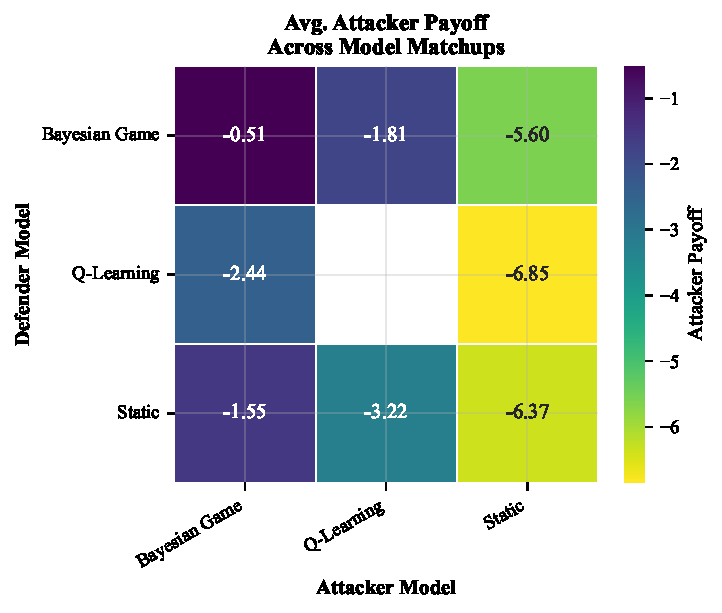
\includegraphics[width=0.45\textwidth]{fig_atk_payoff_heatmap.pdf}
  \caption{Interval-averaged attacker payoff across strategy matchups.}
  \label{fig:atk_payoff_heatmap}
\end{figure}

\begin{figure}[htbp]
  \centering
  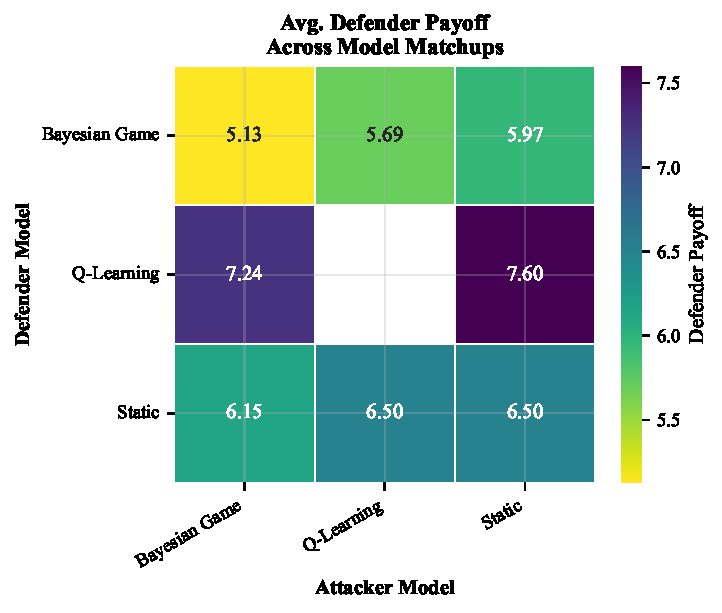
\includegraphics[width=0.45\textwidth]{fig_def_payoff_heatmap.pdf}
  \caption{Interval-averaged defender payoff across strategy matchups.}
  \label{fig:def_payoff_heatmap}
\end{figure}

\begin{figure}[htbp]
  \centering
  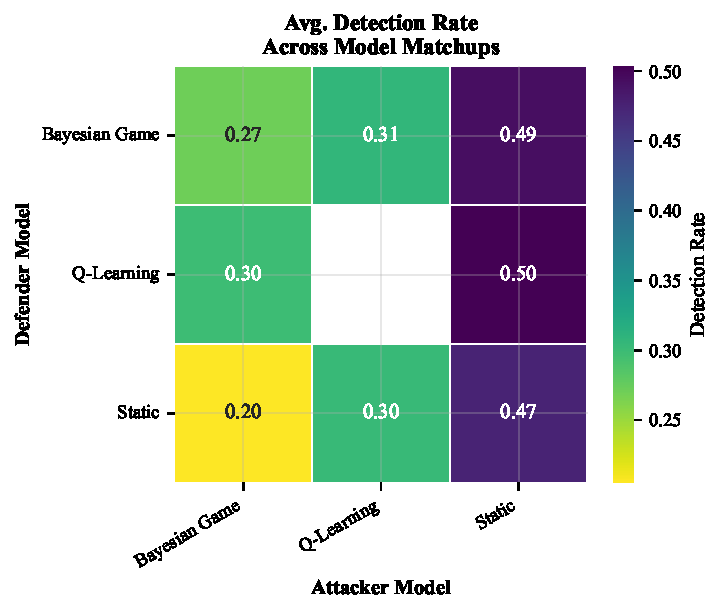
\includegraphics[width=0.45\textwidth]{fig_detection_heatmap.pdf}
  \caption{Detection rate across strategy matchups.}
  \label{fig:detection_heatmap}
\end{figure}

\begin{figure}[htbp]
  \centering
  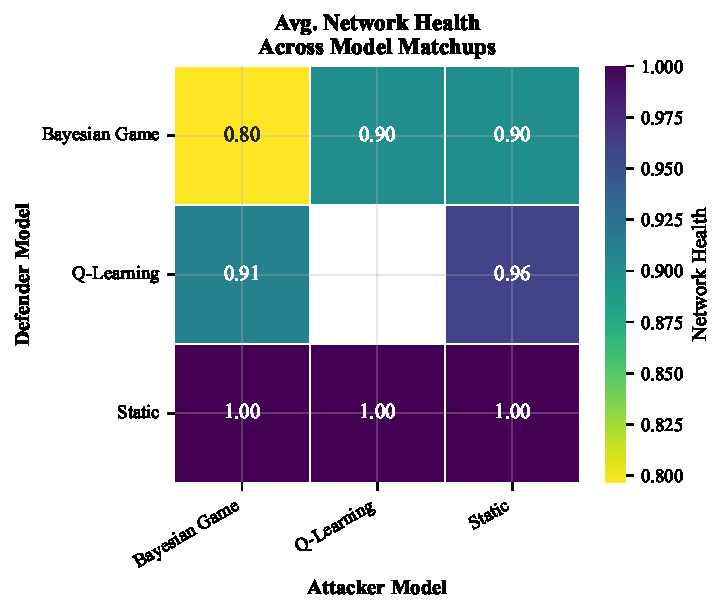
\includegraphics[width=0.45\textwidth]{fig_net_health_heatmap.pdf}
  \caption{Network health across strategy matchups.}
  \label{fig:health_heatmap}
\end{figure}
%--- End Figures ---

\subsection{Convergence Analysis}
Figure~\ref{fig:conv_db} illustrates defender payoff trajectories over time for Q-Learning and Bayesian strategies. Q-Learning defenders show rapid early improvement due to exploratory behavior, but plateau after step 150, often converging to locally optimal policies. In contrast, Bayesian defenders exhibit a slower but more stable convergence pattern, achieving higher long-term payoff with minimal inter-trial variance. This behavior reflects the advantage of equilibrium-driven decision-making under uncertainty~\cite{zeng2023comparison}.

\begin{figure}[htbp]
  \centering
  \includegraphics[width=0.45\textwidth]{fig_def_convergence.pdf}
  \caption{Defender payoff convergence: Q-Learning vs Bayesian Game.}
  \label{fig:conv_db}
\end{figure}

\subsection{Boxplot Comparisons}
Figure~\ref{fig:def_box} shows the distribution of final defender payoffs at $T=500$ across defender strategies (hue indicates attacker type). Bayesian defenders exhibit tighter payoff distributions (IQR = 0.2) compared to Q-Learning (IQR = 0.35), indicating more stable and predictable behavior. Additionally, the median payoff for Bayesian strategies is higher in all attacker pairings, underscoring their robustness against adversarial variability~\cite{zeng2023comparison}.

\begin{figure}[htbp]
  \centering
  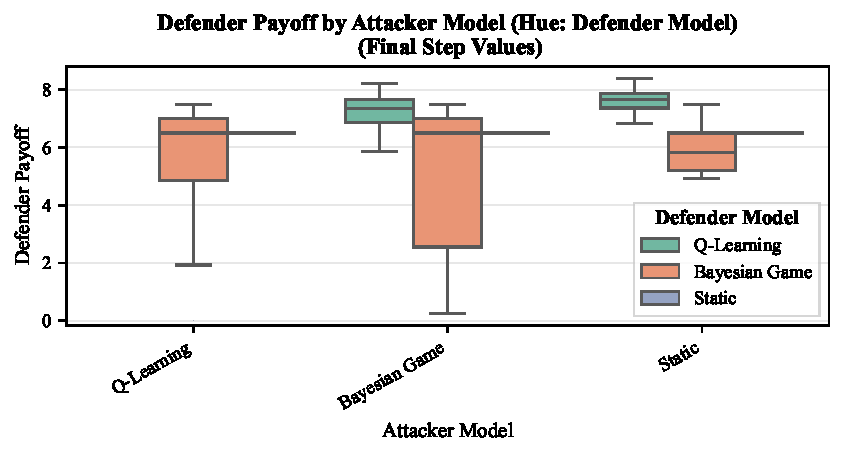
\includegraphics[width=0.45\textwidth]{fig_def_payoff_boxplot.pdf}
  \caption{Distribution of final defender payoffs across strategies.}
  \label{fig:def_box}   
\end{figure}

\subsection{Statistical Analysis}
Table~\ref{tab:anova} summarizes one-way ANOVA results on metrics at the final interval ($\tau=500$). All metrics show $p<0.001$, confirming significant differences between strategy matchups. The high F-statistics for attacker payoff and detection rate indicate that the choice of defense strategy has a substantial influence on these outcomes. The effect size for attacker payoff ($\eta^2 \approx 0.68$) further suggests that the strategy type accounts for a large portion of the observed variance.

\begin{table}[htbp]
  \centering
  \caption{ANOVA results across strategy matchups for key metrics.}
  \label{tab:anova}
  \begin{tabular}{lccc}
    \toprule
    \textbf{Metric} & \textbf{F-Statistic} & \textbf{p-value} & \textbf{Significance} \\
    \midrule
    Attacker Payoff & 249.354 & $<$0.001 & Yes \\
    Defender Payoff & 25.065  & $<$0.001 & Yes \\
    Network Health  & 6.375   & $<$0.001 & Yes \\
    Detection Rate  & 90.339  & $<$0.001 & Yes \\
    \bottomrule
  \end{tabular}
\end{table}

%======================== 6. Discussion ========================
\section{Discussion}

Our comparative results indicate that Bayesian game-theoretic defenses offer consistently robust performance with low variance, making them well-suited for IoT applications that require predictable security guarantees. Among all evaluated metrics, the most pronounced improvement is observed in detection rate, where Bayesian defenders outperform Q-Learning counterparts by approximately 7\%. This reliability stems from the model's use of prior beliefs and equilibrium reasoning, which ensures stability even under uncertainty~\cite{zeng2023comparison}.

However, the computational overhead of belief updates and equilibrium computation may hinder real-time deployment in larger or more dynamic networks, particularly on constrained edge devices. In contrast, Q-Learning defenders demonstrate fast initial adaptation to attacker behavior, achieving higher early-stage payoffs. Yet, their long-term performance often degrades due to convergence to local optima, as also noted in recent studies on adversarial instability in RL-based security~\cite{wang2023adversarial}.

This trade-off reveals complementary strengths between the two approaches. We propose that future defenses may benefit from hybrid architectures that initialize reinforcement learning (RL) agents using prior-informed strategies derived from Bayesian equilibrium policies. Such designs could provide fast adaptation in early rounds while converging toward stable, high-performance policies over time.

\paragraph{Resource Constraints and Real-World Deployment}

Although our simulations were conducted on a general-purpose laptop, the algorithms were intentionally designed with computational efficiency in mind. For real-world IoT deployments, further evaluation on hardware platforms such as Raspberry Pi or ESP32 would help assess energy usage, memory footprint, and real-time feasibility. This concern is particularly relevant given the adversarial challenges faced by RL agents in constrained environments~\cite{wang2023adversarial}.

%=============== 7. Conclusion and Future Work =====================
\section{Conclusion and Future Work}

This paper presented a comparative study of two adaptive jamming defense strategies—Bayesian game-theoretic reasoning and Q-Learning reinforcement learning—within the context of resource-constrained IoT networks. Our simulations demonstrated that Bayesian strategies yield more stable and predictable performance across metrics such as detection rate, attacker payoff, and network health, while Q-Learning offers faster initial adaptation at the cost of long-term consistency.

The findings highlight a core trade-off between stability and adaptability, suggesting that future systems may benefit from hybrid designs that combine the strengths of both approaches~\cite{khoury2020hybrid}. The modular simulator and all experimental artifacts have been made publicly available to facilitate reproducibility and further exploration.

Future work will explore several promising directions: scaling to larger topologies ($n > 50$), integrating deep RL for generalization in high-dimensional state spaces, and conducting hardware-in-the-loop evaluations using real IoT nodes. Additionally, we plan to benchmark both strategies on low-power embedded platforms to evaluate energy efficiency, memory usage, and responsiveness—further bridging the gap between theory and real-world deployment.

%======================== Code Availability ========================
\section*{Code Availability}
The full code, including \texttt{core\_sim.py}, \texttt{run\_experiments.py}, and \texttt{plot\_results.py}, is available at our \href{https://github.com/UmarYaksambi/Adaptive-Defense-Wireless-Networks}{GitHub Repository}.

Detailed instructions for replication and dataset generation are provided.

%======================== Appendix ========================
\appendix
\section{Additional Figures}
The following supplementary figures provide further insight into the experimental results and analysis discussed in the main text.

\begin{figure}[h!]
    \centering
    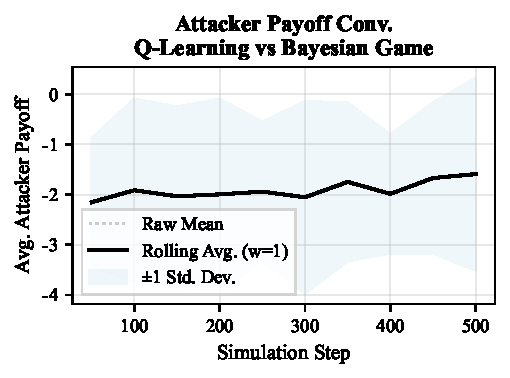
\includegraphics[width=0.9\linewidth]{figures/appendix/fig_atk_convergence.pdf}
    \caption{Attacker payoff convergence (all matchups or aggregated).}
\end{figure}

\begin{figure}[h!]
    \centering
    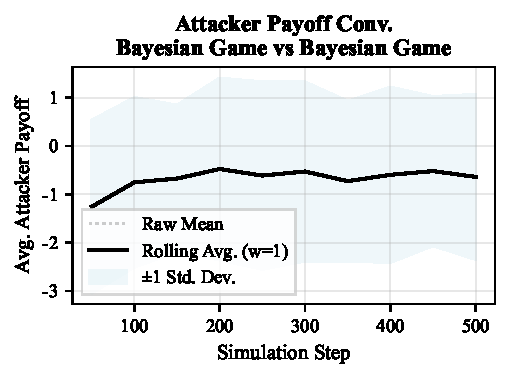
\includegraphics[width=0.9\linewidth]{figures/appendix/fig_atk_convergence_Bayesian_Game_vs_Bayesian_Game.pdf}
    \caption{Attacker payoff convergence: Bayesian Game vs Bayesian Game.}
\end{figure}

\begin{figure}[h!]
    \centering
    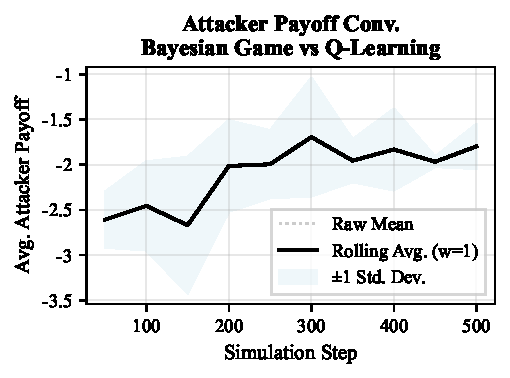
\includegraphics[width=0.9\linewidth]{figures/appendix/fig_atk_convergence_Bayesian_Game_vs_Q_Learning.pdf}
    \caption{Attacker payoff convergence: Bayesian Game vs Q-Learning.}
\end{figure}

\begin{figure}[h!]
    \centering
    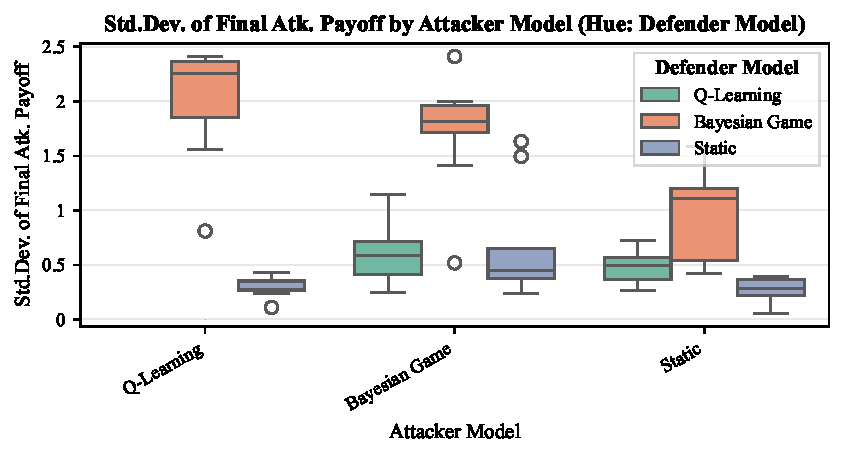
\includegraphics[width=0.9\linewidth]{figures/appendix/fig_atk_payoff_stdev_boxplot.pdf}
    \caption{Standard deviation of attacker payoff (boxplot).}
\end{figure}

\begin{figure}[h!]
    \centering
    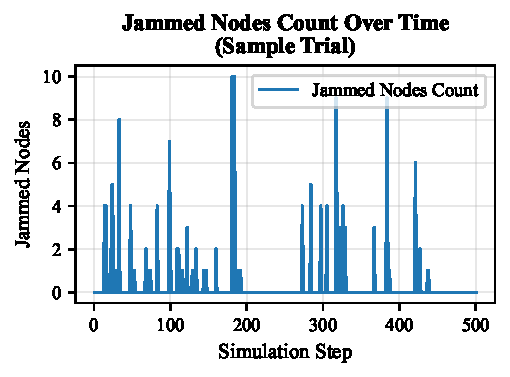
\includegraphics[width=0.9\linewidth]{figures/appendix/fig_collision_count_over_time.pdf}
    \caption{Collision count over time.}
\end{figure}

\begin{figure}[h!]
    \centering
    \includegraphics[width=0.9\linewidth]{figures/appendix/fig_def_convergence.pdf}
    \caption{Defender payoff convergence (all matchups or aggregated).}
\end{figure}

\begin{figure}[h!]
    \centering
    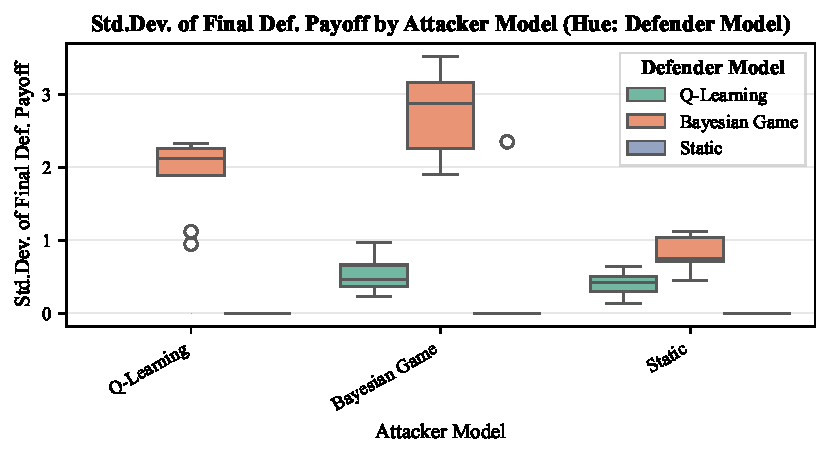
\includegraphics[width=0.9\linewidth]{figures/appendix/fig_def_payoff_stdev_boxplot.pdf}
    \caption{Standard deviation of defender payoff (boxplot).}
\end{figure}

\begin{figure}[h!]
    \centering
    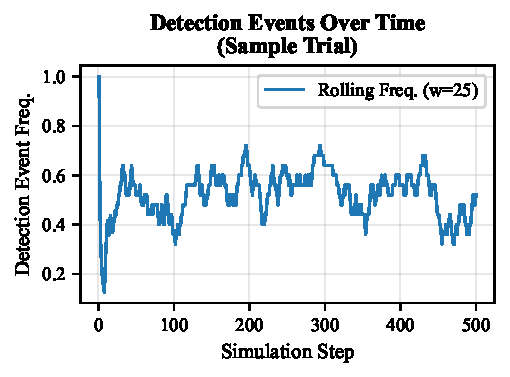
\includegraphics[width=0.9\linewidth]{figures/appendix/fig_detection_events_over_time.pdf}
    \caption{Detection events over time.}
\end{figure}

\begin{figure}[h!]
    \centering
    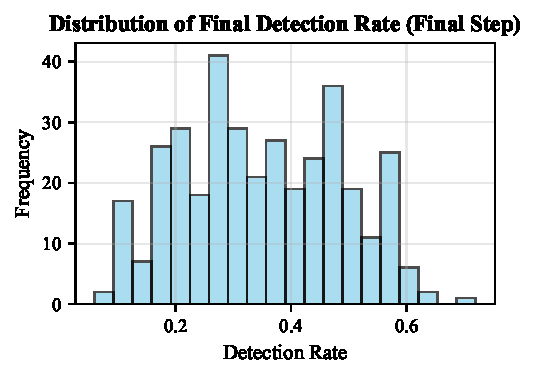
\includegraphics[width=0.9\linewidth]{figures/appendix/fig_detection_variance_histogram.pdf}
    \caption{Histogram of detection rate variance.}
\end{figure}

\begin{figure}[h!]
    \centering
    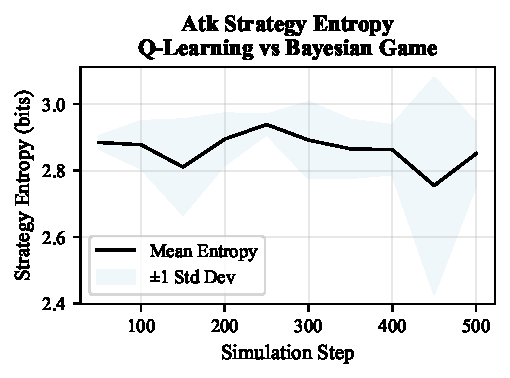
\includegraphics[width=0.9\linewidth]{figures/appendix/fig_entropy_atk_Q_learning.pdf}
    \caption{Entropy of attacker strategies (Q-Learning).}
\end{figure}

\begin{figure}[h!]
    \centering
    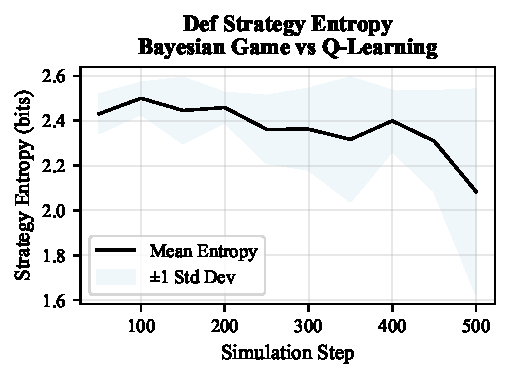
\includegraphics[width=0.9\linewidth]{figures/appendix/fig_entropy_def_Q_learning.pdf}
    \caption{Entropy of defender strategies (Q-Learning).}
\end{figure}

\begin{figure}[h!]
    \centering
    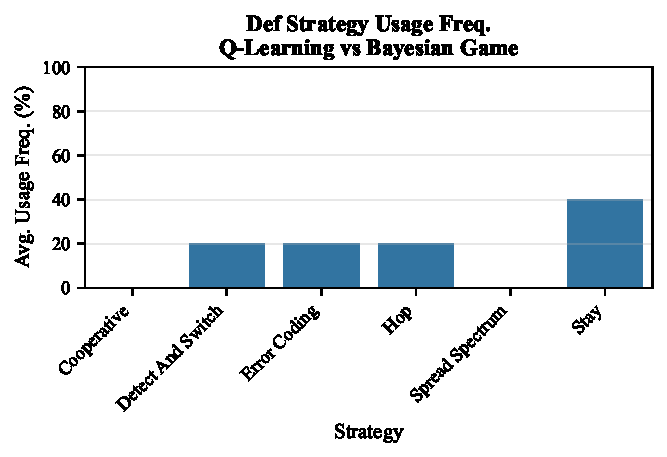
\includegraphics[width=0.9\linewidth]{figures/appendix/fig_freq_def_QL_vs_Bayes.pdf}
    \caption{Defender strategy/channel usage frequency (Q-Learning vs Bayesian).}
\end{figure}

\begin{figure}[h!]
    \centering
    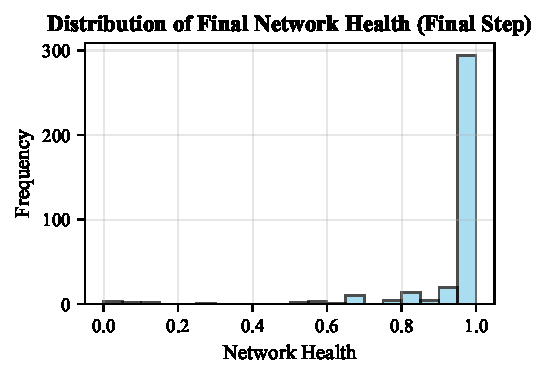
\includegraphics[width=0.9\linewidth]{figures/appendix/fig_health_variance_histogram.pdf}
    \caption{Histogram of network health variance.}
\end{figure}

All supplementary heatmaps (frequency usage distributions and self-play convergence variants) are included in the online repository due to space constraints.

\section{Hyperparameter Grid}
Tested hyperparameter values:
\begin{itemize}
  \item Learning rate $\alpha \in \{0.01,0.05,0.1\}$
  \item Discount factor $\gamma \in \{0.8,0.9,0.99\}$
  \item Exploration $\epsilon_{0}=0.5$, decay $\{0.995,0.998\}$, $\epsilon_{\min}=0.01$
  \item Trials $M=5$, steps $T=500$, logging interval $\tau=50$
\end{itemize}

%======================== References ========================
\bibliographystyle{IEEEtran}
\bibliography{references}

\end{document}